\documentclass[10pt,a4paper]{article}
\usepackage[top=0in, bottom=0.5in,margin=1in, includefoot]{geometry}
\usepackage[utf8]{inputenc}
\usepackage[T1]{fontenc}
\date{}
\author{}
\usepackage{amsmath}
\usepackage{wrapfig}
\usepackage{graphicx}
\usepackage{lineno}
\usepackage{layout}
\setlength{\voffset}{-0.6in}
\textheight = 735pt
\begin{document}
\vspace{-20mm}
\title{\textbf{EE2-08C Numerical Analysis} \\ Group 9\vspace{-17mm}}
\maketitle


\section*{Exercise 3}\vspace{-1mm}

\begin{wrapfigure}{r}{0.5\textwidth}
	\begin{center}
  		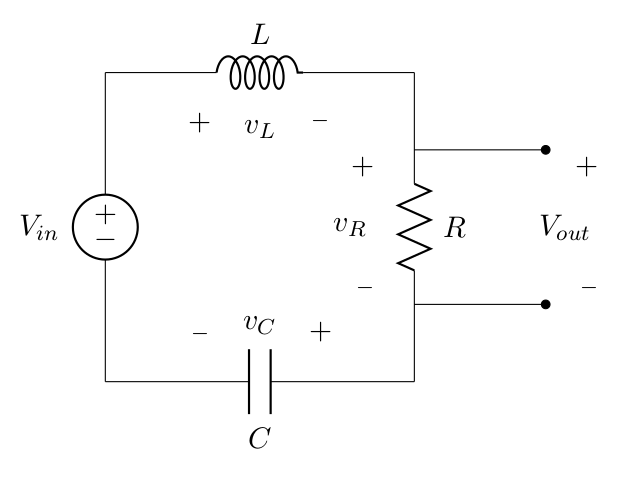
\includegraphics[width=0.48\textwidth]{Ex3_Figs/RLC.png}
	\end{center}
\vspace{-6mm}
  	\caption{RLC Circuit}
  	\label{fig:RLC}
\end{wrapfigure}

From Kirchoff's Voltage Law (KVL) the sum of all the voltages in a closed loop must sum to 0 V. Therefore from this we can derive the equation $V_{in}(t) = v_L(t)+v_R(t)+v_C(t)$. All of the voltages in the closed loop current which flows through them, all being equal to the inductor current. The voltage across a conductor is the inductance multiplied by the derivative of it's current, the voltage across the resistor is equal to it's resistance multiplied by the current travelling through it and the voltage across the capacitor is the charge held within the capacitor divided by the capacitance of the capacitor. Substituting these characteristics into the equation above gives us the equation:

\[ L \frac{d}{dt}i_L(t) + R i_L(t) + \frac{1}{C}\int\limits_0^t i_L(t) \ dt = V_{in}(t)\]

Substituting $i_L(t)$ for $\frac{d}{dt}q_C(t)$ you make the equation:

\[ L \frac{d^2}{dt^2}q_C(t) + R\frac{d}{dt}q_C(t) + \frac{1}{C}q_C(t) = V_{in}(t)\]

We were then able to turn this second order ODE into a set of 2 coupled first order ODEs through the use of equating $q_C'(t)$ = $y(t)$ and substituting $q_C(t)$ for $x(t)$ we have the coupled equations:

\[y(t) = x'(t) \text{\hspace{5mm}and \hspace{5mm}}y'(t) = \frac{1}{L}[V_{in}(t)  - Ry(t) - \frac{1}{C}x(t)] \]

For our project we have values:

\[R = 250 \Omega, C = 3 \mu F , L = 650 mH, i_L(0) = 0 \hspace{2mm} (y_0) \text{\hspace{2mm}and\hspace{2mm}} q_C(0) = 500nC \hspace{2mm} (x_0).\]

Now that we have these two equations we are able to implement them into MATLAB scripf called 'RLC\_script.m` by defining them as:

\begin{verbatim}
R = 250; L = 650*10^-3; C = 3*10^-6; %Impedance values for the components
w1 = 2*pi*500; %frequency for the 500 Hz sinusoid
w2 = 2*pi*100; %frequency for the sinusoid
w3 = 2*pi*5; %frequency for the sinusoid
tc = 3*10^-6; %tau for the exponential decay input
y0 = 0; x0 = 500*10^-9; t0 = 0; %Initial conditions y = iL, x =qC and t = time
h = 0.00001; %step size
tf = 0.03; %final condition
func1 = @(x, y, t) y; %y = q'
func2 = @(x, y, t) (Vin - R*y - x/C)/L; %the second coupled equation
\end{verbatim}

To now evaluate these coupled equations, we use the Runge Kutta 4th order 3/8 algorithm to use these two coupled equations to estimate the next point of the current $i_L$ and the charge $q_C$. The algorithm is:

\[f_1(x,y,t) = y \hspace{3mm} f_2(x,y,z) = \frac{1}{L}[V_{in}(t) - Ry - \frac{x}{C}]\]
\[k1_x = hf_1(x_i,y_i,t_i) \hspace{3mm} k1_y = hf_2(x_i,y_i,t_i)\]
\[k2_x = hf_1(x_i+\frac{k1_x}{3},y_i+\frac{k1_y}{3},t_i+\frac{h}{3}) \]
\[k2_y = hf_2(x_i+\frac{k1_x}{3},y_i+\frac{k1_y}{3},t_i+\frac{h}{3})\]
\[k3_x = hf_1(x_i-\frac{k1_x}{3}+k2_x,y_i-\frac{k1_y}{3}+k2_y,t_i+\frac{2h}{3}) \]
\[k3_y = hf_2(x_i-\frac{k1_x}{3}+k2_x,y_i-\frac{k1_y}{3}+k2_y,t_i+\frac{2h}{3})\]
\[k4_x = hf_1(x_i+k1_x-k2_x+k3_x,y_ik1_y-k2_y+k3_y,t_i+h) \]
\[k4_y = hf_2(x_i+k1_x-k2_x+k3_x,y_ik1_y-k2_y+k3_y,t_i+h)\]
\[x_{i+1} =x_i+\frac{k1_x+3k2_x+3k3_x+k4_x}{8} \hspace{3mm} y_{i+1} =y_i+\frac{k1_y+3k2_y+3k3_y+k4_y}{8}\]
\[t_{i+1} = t_i + h \hspace{3mm} \text{where h is time step}\]

To implement this into MATLAB we created a function called `RK4second.m' in which would take in the two functions and work out the k efficients for both x and y and from there, work out the next position of the x (charge) and y (current) coordinates.

\begin{verbatim}
function [xout, yout] = RK4second (xin, yin, h, tin, func1, func2)

	k1x = h*feval(func1, xin ,yin, tin); %approx the first consts for RK4th ord 3/8 Method
k1y = h*feval(func2, xin ,yin, tin);
	k2x = h*feval(func1, xin + k1x/3, yin + k1y/3, tin+h/3);
	k2y = h*feval(func2, xin + k1x/3, yin + k1y/3, tin+h/3);
	k3x = h*feval(func1, xin  - k1x/3 + k2x, yin - k1y/3 + k2y, tin+2*h/3);
	k3y = h*feval(func2, xin  - k1x/3 + k2x, yin - k1y/3 + k2y, tin+2*h/3);
	k4x = h*feval(func1, xin + k1x - k2x + k3x, yin + k1y - k2y + k3y, tin+h);
k4y = h*feval(func2, xin + k1x - k2x + k3x, yin + k1y - k2y + k3y, tin+h);

	xout = xin + (k1x + 3*k2x + 3*k3x + k4x)/8;
	yout = yin + (k1y + 3*k2y + 3*k3y + k4y)/8;
end
\end{verbatim}

This takes in the present value of current and charge a certain time, the time position, the step time and the two functions to evaluate and approximate the next point, which is then outputted at the end.

\begin{wrapfigure}{r}{0.5\textwidth}
	\begin{center}
  		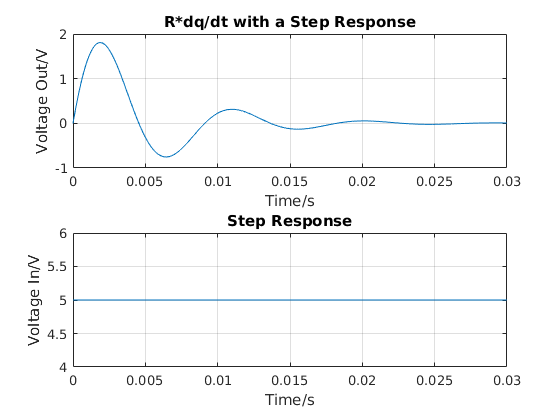
\includegraphics[width=0.49\textwidth]{Ex3_Figs/Step.png}
	\end{center}
	\vspace{-6mm}
  	\caption{$V_{in}(t)= 5$}
  	\label{fig:ex3g1}
\end{wrapfigure}

The sine wave

\begin{wrapfigure}{r}{0.5\textwidth}
	\begin{center}
  		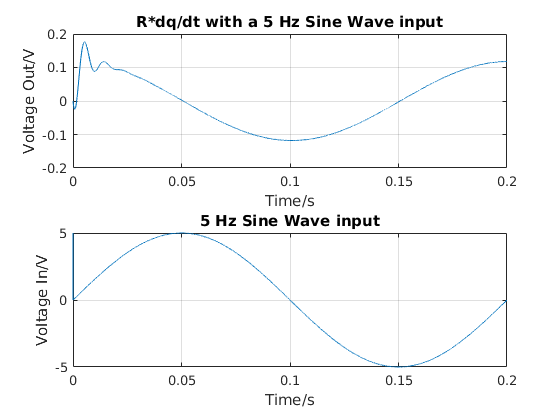
\includegraphics[width=0.48\textwidth]{Ex3_Figs/5Sine2.png}
	\end{center}
	\vspace{-6mm}
  	\caption{$V_{in}(t)= 5sin(2 \pi 5t)$}
  	\label{fig:ex3g2}
\end{wrapfigure}

\begin{wrapfigure}{r}{0.5\textwidth}
	\begin{center}
  		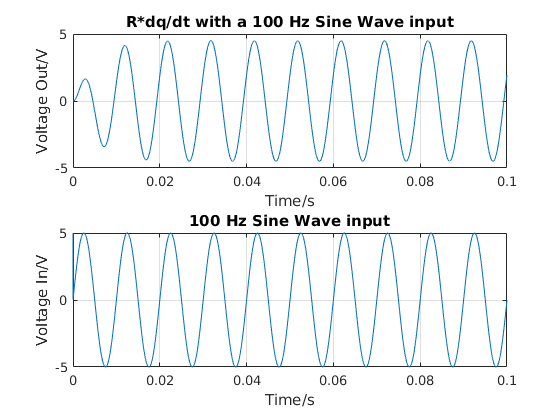
\includegraphics[width=0.48\textwidth]{Ex3_Figs/100Sine.png}
	\end{center}
	\vspace{-6mm}
  	\caption{$V_{in}(t)= 5sin(2 \pi 100t)$}
  	\label{fig:ex3g3}
\end{wrapfigure}

\begin{wrapfigure}{r}{0.5\textwidth}
	\begin{center}
  		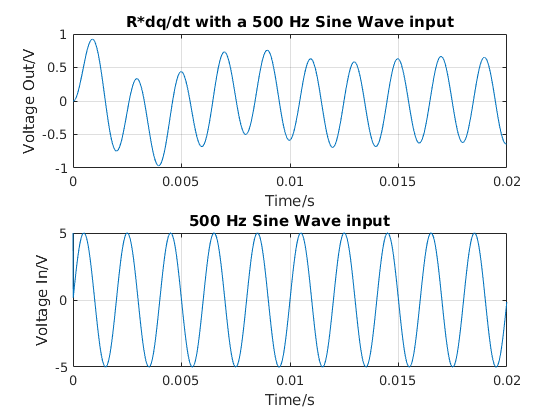
\includegraphics[width=0.48\textwidth]{Ex3_Figs/500Sine.png}
	\end{center}
	\vspace{-6mm}
  	\caption{$V_{in}(t)= 5sin(2 \pi 500t)$}
  	\label{fig:ex3g4}
\end{wrapfigure}

\begin{wrapfigure}{r}{0.5\textwidth}
	\begin{center}
  		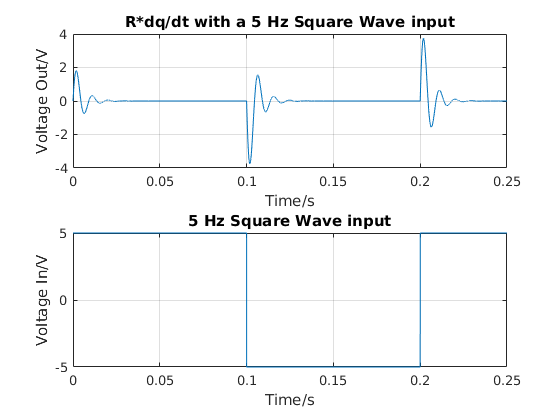
\includegraphics[width=0.48\textwidth]{Ex3_Figs/5Squ1.png}
	\end{center}
	\vspace{-6mm}
  	\caption{$V_{in}(t)= 5square(2 \pi 5t)$}
  	\label{fig:ex3g5}
\end{wrapfigure}

\begin{wrapfigure}{r}{0.5\textwidth}
	\begin{center}
  		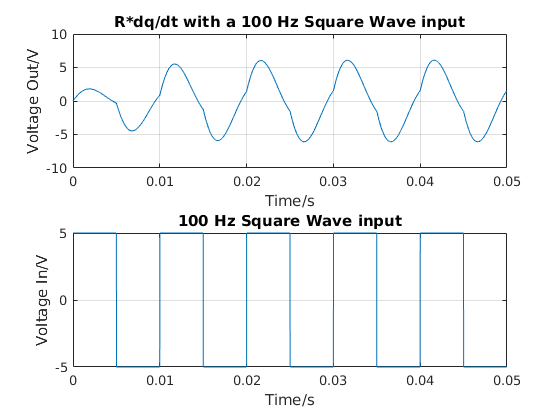
\includegraphics[width=0.48\textwidth]{Ex3_Figs/100Squ1.png}
	\end{center}
	\vspace{-6mm}
  	\caption{$V_{in}(t)= 5square(2 \pi 100t)$}
  	\label{fig:ex3g6}
\end{wrapfigure}

\begin{wrapfigure}{r}{0.5\textwidth}
	\begin{center}
  		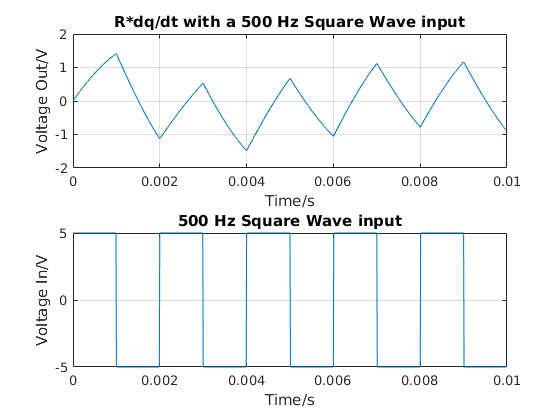
\includegraphics[width=0.48\textwidth]{Ex3_Figs/500Squ1.png}
	\end{center}
	\vspace{-6mm}
  	\caption{$V_{in}(t)= 5square(2 \pi 500t)$}
  	\label{fig:ex3g7}
\end{wrapfigure}

\begin{wrapfigure}{r}{0.5\textwidth}
	\begin{center}
  		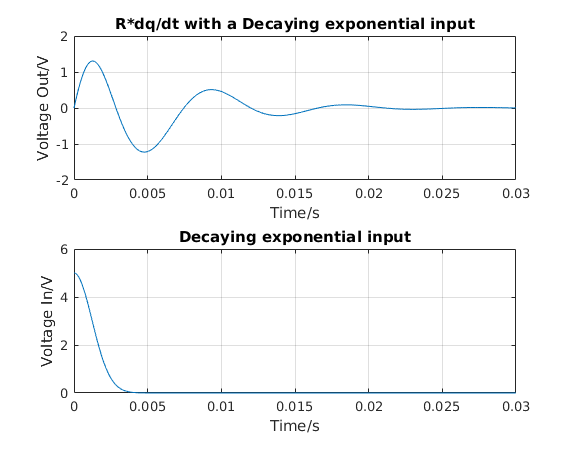
\includegraphics[width=0.48\textwidth]{Ex3_Figs/DecExp.png}
	\end{center}
	\vspace{-6mm}
  	\caption{$V_{in}(t)= 5e^{\frac{-t^2}{\tau_C}}$}
  	\label{fig:ex3g7}
\end{wrapfigure}

\end{document}
